%% Author's version (de-anonymised). Accepted at ICAIF '26, withdrawn before publication.
%% Compile on Overleaf: acmart is preinstalled there; it is not installed locally,
%% so this file has never been compiled. Expect small first-build fixes.
\documentclass[sigconf,nonacm]{acmart}

\AtBeginDocument{%
  \providecommand\BibTeX{{\normalfont B\kern-0.5em{\scshape i\kern-0.25em b}\kern-0.8em\TeX}}}
%% acmart warns that the ACM reference format is mandatory for papers over one
%% page, so printacmref is left at its default rather than suppressed.
\setcopyright{none}
\copyrightyear{2026}
\acmYear{2026}
\acmConference[ICAIF '26]{ACM International Conference on AI in Finance}{November 14--17, 2026}{Milan, Italy}

%% booktabs and graphicx are already loaded by acmart; do not re-require them.

\begin{document}

\title{The Price of Evaluation Choices in Portfolio Backtests}
\titlenote{Author's version. Accepted at the ACM International Conference on AI in Finance (ICAIF '26), Milan; withdrawn by the author before publication. Not published elsewhere.}

\author{Ayush Sunil Munot}
\affiliation{\institution{Indian Institute of Technology Kharagpur}\city{Kharagpur}\country{India}}
\email{munotayush6@gmail.com}

\begin{abstract}
A backtest reports a number, but that number depends on choices the reader never
sees: which baseline was used, over which dates, at which trading cost, and at
which random seed; we measure what those choices are worth. We first build a set
of regime-aware, graph-based and neural portfolio methods inside one causal,
cost-aware pipeline, and find that no method beats a simple baseline out of
sample. That failure gives us a test bed with a known ground truth. None of the
methods has an edge, so any performance still visible in these runs comes from
how the results were reported. Across 345 manifest-backed runs on four fixed-instrument panels and
two markets, we hold the data, allocator, cost model and execution rule fixed
and change one reporting choice at a time. Ignoring trading costs adds $0.232$
to the Sharpe ratio of a model that trades 56\% of the portfolio a month, but
only $0.010$ to equal weight, so the effect grows with turnover. A benchmark
measured over different dates adds $0.493$ to the reported figure, and reporting
a single favourite baseline rather than the full set adds $0.070$ while
reversing the sign of the conclusion. An uncorrected best-of-family $p$-value understates the
corrected one by up to $0.321$. We then pre-registered a prediction of failure and tested it on a sealed panel sharing no instrument with the
development data. The prediction held, and the trading-cost result repeated out
of sample.
\end{abstract}

\begin{CCSXML}
<ccs2012>
   <concept>
       <concept_id>10010147.10010257</concept_id>
       <concept_desc>Computing methodologies~Machine learning</concept_desc>
       <concept_significance>500</concept_significance>
       </concept>
   <concept>
       <concept_id>10010147.10010257.10010339</concept_id>
       <concept_desc>Computing methodologies~Cross-validation</concept_desc>
       <concept_significance>300</concept_significance>
       </concept>
   <concept>
       <concept_id>10002950.10003648.10003688.10003693</concept_id>
       <concept_desc>Mathematics of computing~Time series analysis</concept_desc>
       <concept_significance>300</concept_significance>
       </concept>
   <concept>
       <concept_id>10002950.10003648.10003688.10003691</concept_id>
       <concept_desc>Mathematics of computing~Regression analysis</concept_desc>
       <concept_significance>100</concept_significance>
       </concept>
 </ccs2012>
\end{CCSXML}

\ccsdesc[500]{Computing methodologies~Machine learning}
\ccsdesc[300]{Computing methodologies~Cross-validation}
\ccsdesc[300]{Mathematics of computing~Time series analysis}
\ccsdesc[100]{Mathematics of computing~Regression analysis}

\keywords{portfolio optimisation, backtest overfitting, multiple testing,
reproducibility, regime models, graph neural networks}

% The generated CCS line has no break point within TeX's normal tolerance and
% sets 13pt overfull without emergency stretch; the group keeps the stretch out
% of body paragraphs.
{\setlength{\emergencystretch}{3em}\maketitle}

\section{Introduction}

Many papers report strong risk-adjusted returns for regime-aware and
graph-neural portfolio methods. We set out to reproduce that kind of result. To
make the comparison fair, we built all of them inside one pipeline, so they see
the same data at the same time and send their output through a shared allocator
and backtester. No method can look better simply because
it was given easier conditions.

Nine candidates failed that test: soft-regime conditional covariance, an
uncertainty-aware hidden Markov risk model, a group-aware covariance variant,
edge-masked graph attention, a training objective based on the information
coefficient (IC),
probability-gated expert heads, direct concatenation of regime probabilities, a
VIX-conditioned regime model, and a dynamic graph-temporal transformer. Each was
compared against conventional allocators on held-out data, and none cleared its
pre-declared release gate (Table~\ref{tab:ladder}).

When the dynamic model is trained for the twenty epochs its configuration
declares, it reproduces the published pattern, reaching a five-seed median
Sharpe of $0.930$ on the development window against $0.792$ for equal weight.
The same runs evaluated on held-out data give $0.604$ against $0.718$.
Section~\ref{sec:inflation} traces how much of the development-window advantage
each reporting choice supplied.

These failures give the rest of the paper a fixed reference point. None of the
methods has an edge, so the true value of any advantage a backtest of them
reports is zero, and an advantage that still appears in a table was supplied by
the evaluation rather than by a method. Reporting choices can therefore be
measured directly. Holding the panel, the strategy, the allocator, the cost
model and the execution rule fixed, we change one reporting choice at a time and
record what happens to the reported number. We call that change \emph{protocol
inflation}.

Our contributions are:

\begin{enumerate}
\item An audited benchmark of 345 manifest-backed causal runs across four
  fixed-instrument panels and two markets, under one shared allocator, cost
  model and release gate.
\item A measurement of protocol inflation. We price six common reporting
  choices across fourteen single-choice cells of Table~\ref{tab:inflation},
  changing one thing at a time and pairing each with a control where one
  exists, plus a fifteenth cell that compounds three of them.
\item A confirmation test on a sealed panel that shares no instrument with the
  development data. We recorded our prediction, which was that the methods would
  fail, before opening it.
\item A reproducibility harness that blocks rather than guesses when something
  is missing, and a demonstration that the whole confirmation cycle re-runs to
  identical numbers.
\end{enumerate}

Our claims are about measurement rather than investment. Each number in this
paper prices an evaluation choice, and that price is a property of the protocol
rather than of any method's merit. The paper accordingly contains no
investable result. The compound cell of Table~\ref{tab:inflation}, which
reports a Sharpe of $1.095$, adjusts to $0.604$ and trails equal weight's
$0.718$ over the same dates.

\section{Related Work}

\begin{figure*}[t]
\centering
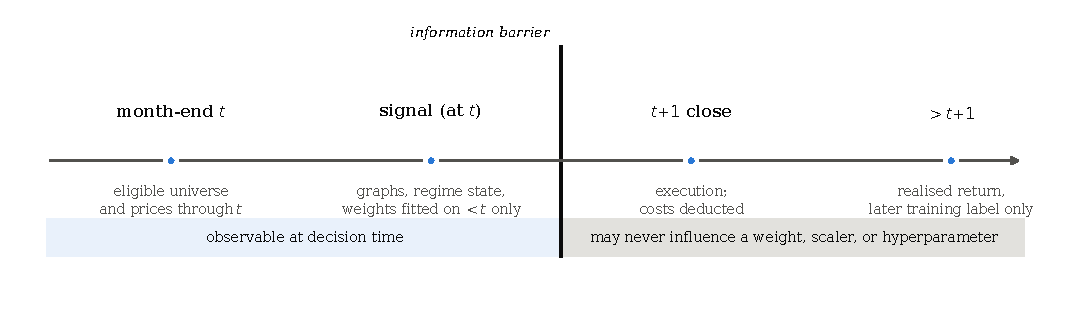
\includegraphics[width=\textwidth]{figures/timeline.pdf}
\caption{The causal decision timeline. At month-end $t$ the pipeline sees only
data through $t$; graphs, regime states, scalers and weights are fitted strictly
before $t$; execution happens at the following close with costs deducted; the
realised return may enter only as a later training label. No scaler, graph edge,
regime feature, hyperparameter, membership record or normalisation statistic may
cross the barrier.}
\Description{A left-to-right timeline with four marked stops: month-end t, the
signal, the t plus one close, and dates after t plus one. A vertical information
barrier sits between the signal, which is computed at month-end t, and the
execution close. The region left of the
barrier is labelled observable at decision time; the region right of it is
labelled as never permitted to influence a weight, scaler, or hyperparameter.}
\label{fig:timeline}
\end{figure*}

This paper builds on the literature on data snooping and backtest
overfitting. White's Reality Check~\cite{white2000reality} and Hansen's test for
superior predictive ability~\cite{hansen2005spa} correct a reported edge for the
size of the search that produced it. The deflated Sharpe
ratio~\cite{bailey2014deflated} and the analysis of backtest
overfitting~\cite{bailey2014pseudo} bound how much a reported Sharpe should be
discounted given the number of trials. Harvey, Liu and
Zhu~\cite{harvey2016cross} make the same argument for the cross-section of
expected returns, and Harvey and Liu~\cite{harvey2015backtesting} for
backtesting generally. Arnott, Harvey and Markowitz~\cite{arnott2019protocol}
propose a protocol for machine-learning backtests.

Most of these results are theoretical, showing that a reported figure deserves
a discount and bounding the size of that discount for a given number of trials.
We contribute the empirical counterpart by pricing each individual choice on
runs where the true edge of every method is known to be zero. The two
quantities are complementary rather than competing, since a deflated Sharpe
tells a reader how much to discount a number while our measurements identify
which decision produced it.

Kapoor and Narayanan~\cite{kapoor2023leakage} document leakage as a
reproducibility problem across machine-learning-based science and argue for
treating it as a first-class object of study. We adopt that stance in a
portfolio setting, where leakage is one of several conventions that inflate a
result, and by our measurements not the largest.

Two studies published in 2026 address closely related questions. Zhang et
al.~\cite{zhang2026alpha} construct a one-switch benchmark that isolates
decision-time leakage and measures the alpha it manufactures. Our treatment of
the development-window choice asks a similar question, and we agree with them
that varying one thing at a time is the right experimental form. The differences
are in scope and in the runs being read. Their study isolates leakage, while we
treat it as one of six choices and find its effect uneven. The same boundary
choice is worth $+0.090$ at our frozen training budget and $+0.326$ at the
declared one, so leakage is among the smaller effects in its headline instance
without being small in general.
A leakage benchmark also has to work out how much of an observed edge was real.
Our runs have no edge to divide up, since every method has already failed on
held-out data, so anything recovered from them is an artefact by
construction. Yin et al.~\cite{yin2026implementation} quantify implementation
risk, the divergence between backtested and deployable performance, which is the
mechanism underlying our cost row. We add a measurement of how that distortion
varies between methods. It grows with turnover, and a low-turnover control makes
that growth visible.

On the methods side, DeMiguel, Garlappi and Uppal~\cite{demiguel2009naive}
established that naive diversification is hard to beat. Our ladder relies on
that result and complicates it, since the identity of the winning baseline
changes from one panel to the next. The allocator ladder draws on hierarchical risk
parity~\cite{lopezdeprado2016hrp}, shrinkage
covariance~\cite{ledoit2004wellconditioned} and conditional value-at-risk
optimisation~\cite{rockafellar2000cvar}; the regime models follow
Hamilton~\cite{hamilton1989regime} and Ang and Bekaert~\cite{ang2002regime}. The
candidates we implement follow recent work on graph-attention
portfolios~\cite{korangi2024gat}, multivariate hidden Markov
selection~\cite{majumder2024mhmm}, the implementable efficient
frontier~\cite{jensen2024frontier}, forecast
stabilisation~\cite{barroso2025calm} and machine-learning asset
pricing~\cite{gu2020empirical}.

\section{Experimental Apparatus}
\label{sec:apparatus}


\begin{figure*}[t]
\centering
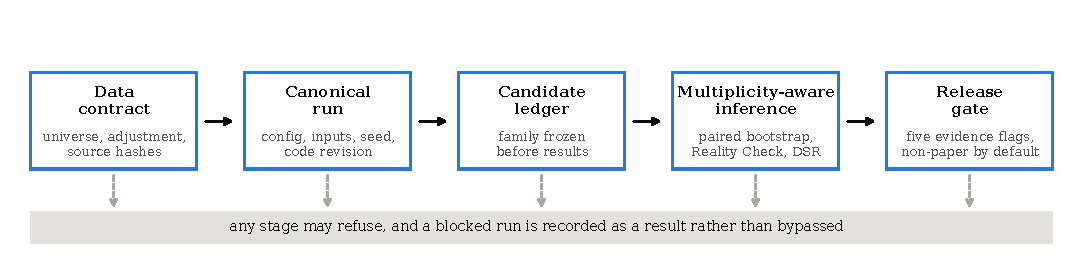
\includegraphics[width=\textwidth]{figures/pipeline.pdf}
\caption{The release path from raw data to a claim. Each stage can only refuse a
run; nothing on the path improves one, so the path acts as a sequence of gates
rather than a processing chain. A blocked run is recorded as a result rather
than bypassed, so a failed candidate remains visible in the record rather than
quietly disappearing.}
\Description{Five boxes connected left to right: data contract, canonical run,
candidate ledger, multiplicity-aware inference, and release gate. Each box lists
what it records or requires. An arrow runs downward from every box into a single
grey band spanning the full width, labelled to say that any stage may refuse and
that a blocked run is recorded as a result rather than bypassed.}
\label{fig:pipeline}
\end{figure*}

\subsection{Causal timeline}
Every method shares the decision timeline drawn in Figure~\ref{fig:timeline}. A
decision made at month-end $t$ may use prices and membership only through $t$.
Graphs, regime states, scalers, model weights and hyperparameters are fitted on
strictly earlier data, and the realised return becomes visible only afterwards,
as a training label. The barrier between what a decision may and may not see is
enforced in code rather than left to convention, so no look-ahead path exists.
Figure~\ref{fig:pipeline} then traces the path a run must travel before it may
support a claim. Every stage on that path can block the run, and no stage can
improve it.

\subsection{Data and protocol}
The panels are fixed lists of exchange-traded funds, declared before any price
was retrieved: 30 US-listed funds from 2010, a wider 50-fund US panel, 12 Indian
funds from 2014, and a second, disjoint list of 30 US-listed funds reserved as
the sealed panel for the confirmation test of
Section~\ref{sec:confirmation}. Prices are daily adjusted closes retrieved through the \texttt{yfinance}
interface, with the retrieval timestamp, library version and response hash
recorded in each run manifest. Decisions are made at each month end, executed at the next close, and
charged 10 basis points one way, with a 10\% cap on any single position.
Rebalancing is monthly except in the frequency robustness cells of
Table~\ref{tab:robustness}, which use quarterly decisions.

\subsection{Metrics}
Sharpe ratios are computed from daily returns net of
transaction costs and annualised by $\sqrt{252}$, with the risk-free rate set to
zero throughout. Our claims concern two readings of the same runs, for which a
common rate offset is second order. Maximum drawdown is taken on the daily
net asset value. Conditional value-at-risk (CVaR) is the mean of the worst 5\% of daily
net returns. Turnover is one-way and reported per executed rebalance. Every
comparison between two strategies uses only the dates both of them realise.

\subsection{Shared allocator}
Every method, conventional or learned,
produces either a cross-sectional score or a covariance matrix. A covariance
matrix is allocated by hierarchical risk parity~\cite{lopezdeprado2016hrp},
which clusters assets on the correlation distance $\sqrt{(1-\rho)/2}$ and splits
capital recursively by inverse cluster variance. A score is allocated by a
long-only mean-CVaR programme~\cite{rockafellar2000cvar} that maximises the
score, taken as the expected-return estimate, less a 5\% conditional
value-at-risk penalty and a turnover penalty on the distance from the current
holding. Both paths are fully invested and capped at
10\% per asset, and both are executed by the same cost-aware backtester, so a
learned method cannot win by being given an easier execution model.

\subsection{Candidates and baselines}
A method is a candidate if it fits a latent
state or trains parameters by gradient descent, and a baseline if it is a
deterministic function of observable returns. This split fixes which methods
enter a family-wise correction, so it was frozen in version control before any
confirmation result was read.

\subsection{Provenance}
Each panel is governed by a versioned contract
declaring its universe, adjustment convention, provider metadata, coverage
requirements and source hashes. Validation precedes every run, and a stale
report is rejected rather than reused.

A canonical run records its
configuration, input hashes, code revision, targets, executions, holdings, daily
net asset value, diagnostics and seed, and every number in this paper resolves
to one of these records.

\subsection{Release gate}
Runs are classified non-paper by default, promotion requires five separate
evidence flags, and the summariser will not export a run that has no
classification. Every run in this study remains unpromoted, which is the state
the design intends. Our claims concern reporting conventions rather than
performance, and the gate keeps the two apart by construction, since nothing in
this study can be exported as a performance result.

\section{Candidate Methods}

\begin{table*}[t]
\centering
\caption{Candidate specifications: mechanism, matched comparator, and what each
comparison isolates. Every candidate sends its output through the shared allocator of
Section~\ref{sec:apparatus}, so a comparison differs only in the component named.
Seeds are the prescribed set $\{7, 17, 29, 43, 59\}$ where a method is stochastic.}
\label{tab:spec}
\footnotesize
\begin{tabular}{p{2.7cm}p{5.1cm}p{4.0cm}p{2.9cm}r}
\toprule
Family & Mechanism & Matched comparator & Isolates & Seeds \\
\midrule
Soft-regime cond.\ covariance & expanding soft $k$-means, 3 states, on four market features; state-mixed shrinkage covariance, 756-session lookback & matched unconditional risk: the same HRP allocation on an unconditional covariance & isolates the state mixture & 1 \\
HMM cond.\ risk (2, 252) & expanding Gaussian HMM, 2 states, 252-session covariance lookback, entropy fallback to unconditional risk & matched HRP-756, the stronger unconditional control; the lookback-matched HRP-252 gives $p{=}0.209$ & isolates state conditioning & 1 \\
9-cell HMM grid & the same model over states $\in\{2,3,4\}$ and lookback $\in\{63,126,252\}$ sessions & matched HRP-756 & prices the search over those two axes & 1 \\
Group-aware cond.\ covariance & as the HMM candidate, but state conditioning retained only within five ex-ante asset groups & matched global-HMM risk & isolates cross-group conditioning & 1 \\
Edge-masked graph attention & attention over the sparsified graph in place of similarity message passing & similarity passing: the same encoder with fixed weights & isolates learned edge weighting & 5 \\
IC training objective & ranking-aligned loss on the cross-sectional information coefficient & likelihood-only: the same model under a Gaussian likelihood & isolates the training objective & 5 \\
Regime-conditioned variants & regime probabilities entering the model by direct concatenation, by gated expert heads, or through a VIX covariate & regime-free model: the same architecture without state input & isolates regime conditioning & 5 \\
Dynamic graph-temporal & partial-correlation graph, 252-session lookback, 5\% edges; 2 graph layers into a 2-layer, 4-head Transformer, $d{=}48$, sequence length 12 & its graph-only and temporal-only ablations, and equal weight & isolates each stage, then the whole model & 5 \\
\bottomrule
\end{tabular}
\end{table*}

\begin{table}[t]
\centering
\caption{Every proposed candidate, its matched comparator, and the one-sided
paired moving-block $p$-value for a positive advantage. The final three rows
are the same model, which beats both of its own ablations and still loses
to equal weight. Thirteen tests cover nine candidates. The
information-coefficient objective appears on two panels, the HMM entry appears with
and without its search correction, and the dynamic model is tested against two
ablations and one baseline. All rows resolve to manifest-backed runs (Section 3).}
\label{tab:ladder}
\footnotesize
\begin{tabular}{llr}
\toprule
Candidate & Compared against & $p$ \\
\midrule
Soft-regime cond.\ covariance & matched uncond.\ risk & $0.909$ \\
HMM cond.\ risk (2, 252) & matched HRP-756 & $0.359$ \\
\quad same, corrected for the 9-cell search & matched HRP-756 & $0.680$ \\
Group-aware cond.\ covariance & matched global-HMM risk & $0.732$ \\
Edge-masked graph attention & similarity passing & $0.474$ \\
IC training objective (US) & likelihood-only & $0.298$ \\
IC training objective (India) & likelihood-only & $0.998$ \\
Probability-gated regime experts & regime-free model & $0.719$ \\
Direct probability concat. & regime-free model & $0.519$ \\
VIX-conditioned regime model & regime-free model & $0.717$ \\
Dynamic graph-temporal, full & own graph-only ablation & $0.007$ \\
\quad same & own temporal-only abl. & $0.023$ \\
\quad same & equal weight & $0.705$ \\
\bottomrule
\end{tabular}
\end{table}


Every candidate was evaluated against a ladder of conventional allocators on
matched dates, using a paired 21-session moving-block bootstrap with 5{,}000
replications~\cite{kunsch1989jackknife,politis1994stationary}. The choice of
block length is not doing the work, since repeating the closest confirmation
comparison at 10, 21, 42 and 63 sessions returns $p$ between $0.131$ and
$0.146$.
Table~\ref{tab:spec} specifies each candidate family, its matched comparator,
and what that comparison isolates; Table~\ref{tab:ladder} lists each test and
the $p$-value it returned. No entry
approaches conventional significance, and the pattern holds across regime
conditioning, graph construction, training objective and architecture alike.
Risk adjustment does not change the picture either, since on the US panels no
strategy earns a statistically significant positive five-factor
alpha~\cite{fama2015fivefactor} under Newey--West standard
errors~\cite{newey1987hac}. We do not run the equivalent regression on the
Indian panel, since the five factors are built for the US cross-section.

A final check rules out undertraining. Our frozen configuration trains the
neural candidate for five epochs, although its declared configuration specifies
twenty, so the failures above could in principle reflect the budget rather than
the architecture. We therefore ran the
declared budget on the development panel across the same five seeds. At twenty
epochs the development
median rises from $0.763$ to $0.930$, moving from below equal weight ($0.792$)
to $0.137$ above it. On held-out data the same runs give $0.604$ against equal
weight's $0.718$, which is $0.115$ below. Quadrupling the training budget therefore adds $0.167$ Sharpe on the development
window and adds nothing out of sample. Differences in this paragraph, as in Table~\ref{tab:inflation}, are
computed from unrounded values. That $0.326$ difference appears as its own row in
Table~\ref{tab:inflation}, and the spread across seeds widens from $0.185$ to
$0.321$. All other results in this paper use the five-epoch setting, the configuration
that entered the confirmation test.

The edge-masked attention model and the graph-temporal transformer are the
graph-neural candidates named in the introduction; both learn by passing
messages over the sparsified partial-correlation graph specified in
Table~\ref{tab:spec}. The last three rows of Table~\ref{tab:ladder} describe the
graph-temporal model and are worth examining separately. The full graph-temporal model beats its own graph-only
($p{=}0.007$) and temporal-only ($p{=}0.023$) ablations, and then loses to equal
weight ($p{=}0.705$). Each component of the model contributes something, and the
model as a whole is still worse than the simplest rule available. An ablation
study cannot detect this by itself, since every comparison it makes is against a
degraded version of the same model.

\section{Protocol Inflation}
\label{sec:inflation}

\begin{table*}[t]
\centering
\caption{Measured inflation from each evaluation choice, grouped by the choice
isolated. Each row reads the same runs twice, holding the panel, strategy, allocator,
cost model and execution rule fixed. Rows marked \emph{sealed} were computed on the
confirmation panel, which had never been examined when the earlier rows were produced.
Inflation is the reported value minus the adjusted one, computed from unrounded values;
columns are rounded to three decimals, so a difference taken from them can disagree in the
last digit. The search-multiplicity group reports $p$-values rather than Sharpe
ratios, so its inflation is a difference in $p$. Sharpe cells aggregate seeds by the
estimator the frozen protocol declared, mean at five epochs and median in the
declared-budget experiment.}
\label{tab:inflation}
\small
\begin{tabular}{p{2.6cm}p{5.0cm}p{4.2cm}rrr}
\toprule
Choice & Panel / strategy & Reading & Reported & Adjusted & Inflation \\
\midrule
Development boundary & US 30-ETF: Causal dynamic graph-temporal model, 5 epochs & development vs held out & $0.775$ & $0.685$ & $\mathbf{+0.090}$ \\
 & US 30-ETF, declared 20-epoch training budget: Dynamic graph-temporal, 5 seeds (equal weight: 0.792 development, 0.718 outer) & development vs held out & $0.930$ & $0.604$ & $\mathbf{+0.326}$ \\
\addlinespace[2pt]
Seed selection & US 30-ETF: Causal dynamic graph-temporal model, outer window & best seed vs median & $0.734$ & $0.729$ & $\mathbf{+0.005}$ \\
 & US 50-ETF: Causal dynamic graph-temporal model, development window & best seed vs median & $1.261$ & $0.759$ & $\mathbf{+0.502}$ \\
 & Confirmation panel, 2020+ secondary window (sealed): Dynamic graph-temporal; best baseline on this window is 0.737 & best seed vs median & $0.799$ & $0.714$ & $\mathbf{+0.085}$ \\
\addlinespace[2pt]
Trading costs & US 30-ETF: Causal dynamic graph-temporal model (mean one-way turnover 56\%/month) & gross vs net of 10\,bps & $0.731$ & $0.500$ & $\mathbf{+0.232}$ \\
 & US 30-ETF: Equal weight (low-turnover control: the shortcut should barely move it) & gross vs net of 10\,bps & $0.720$ & $0.710$ & $\mathbf{+0.010}$ \\
 & Confirmation panel (US 30-ETF, sealed): Dynamic graph-temporal, seed 7 (48.9\%/month turnover) & gross vs net of 10\,bps & $0.735$ & $0.568$ & $\mathbf{+0.167}$ \\
 & Confirmation panel (US 30-ETF, sealed): Equal weight (low-turnover control: 2.0\%/month) & gross vs net of 10\,bps & $0.680$ & $0.673$ & $\mathbf{+0.007}$ \\
\addlinespace[2pt]
Benchmark choice & Confirmation panel (US 30-ETF, sealed): Dynamic graph-temporal, best seed vs the six pre-declared baselines & one baseline vs ladder & $+0.045$ & $-0.025$ & $\mathbf{+0.070}$\,$\dagger$ \\
\addlinespace[2pt]
Date alignment & Confirmation panel, quarterly rebalance (sealed): Dynamic graph-temporal seed 7 (24-quarter warm-up starts 2020) vs equal weight & own dates vs matched & $+0.538$ & $+0.045$ & $\mathbf{+0.493}$ \\
\addlinespace[2pt]
Search multiplicity & US 30-ETF: HMM cond.\ risk (2, 252), 9-cell grid vs matched HRP-756 control & best cell vs corrected & $0.359$ & $0.680$ & $\mathbf{+0.321}$ \\
 & Confirmation panel (US 30-ETF, sealed): Seven-candidate confirmation family vs strongest baseline & best cell vs corrected & $0.131$ & $0.344$ & $\mathbf{+0.213}$ \\
 & Confirmation panel, 2020+ secondary window (sealed): Seed 7 alone vs the seven-candidate family, against the strongest baseline & best cell vs corrected & $0.065$ & $0.185$ & $\mathbf{+0.120}$ \\
\addlinespace[2pt]
Combined choices & US 30-ETF, declared 20-epoch budget: Development window, best seed, zero costs, against held-out median at 10 bps & three choices at once vs adjusted & $1.095$ & $0.604$ & $\mathbf{+0.491}$ \\
\bottomrule
\end{tabular}
\\[2pt]
\footnotesize $\dagger$ the sign of the conclusion changes, not merely its magnitude.
\end{table*}


\begin{figure*}[t]
\centering
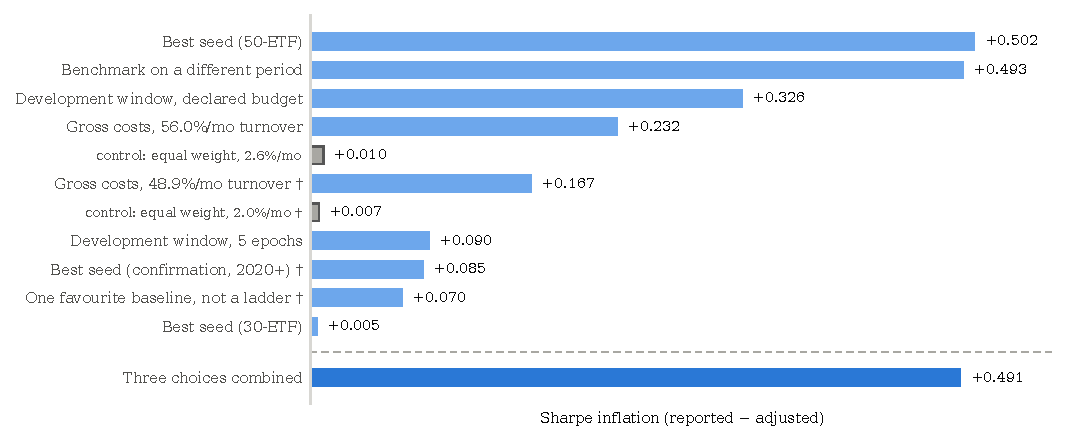
\includegraphics[width=\textwidth]{figures/inflation.pdf}
\caption{Measured inflation per evaluation choice. Grey bars are low-turnover
controls, drawn directly beneath the high-turnover cell they pair with; the
same choice barely moves them, and that contrast is the evidence that the
convention is not neutral. The dashed rule separates the compound reading, drawn in a
deeper blue because it combines three choices rather than pricing a single one.
Rows marked $\dagger$ come from the confirmation panel, which stayed sealed
until every configuration was frozen (Section~\ref{sec:confirmation}).}
\Description{A horizontal bar chart of the measured evaluation choices, ordered
by size. Each gross-cost bar has its low-turnover control drawn directly beneath
it in grey, near zero. A dashed rule separates the bottom bar, drawn in a deeper
blue because it combines three choices at once, from the mid-blue single-choice
bars above it.}
\label{fig:inflation}
\end{figure*}

Table~\ref{tab:inflation} and Figure~\ref{fig:inflation} give the main result.
Each row reads the same runs twice. The Reported column applies one favourable
evaluation choice, and the Adjusted column removes it. Nothing else changes
between the two columns, so the gap between them is the price of that single
choice.

\subsection{Trading costs}
Leaving costs out adds $0.232$ to the
Sharpe ratio of a model that trades 56\% of the portfolio a month. The same
omission adds only $0.010$ to equal weight, which trades 2.6\%. The effect
therefore depends on how much a strategy trades. In most papers the method that
trades most is the one being put forward, so the omission helps the proposal
more than the baseline. The same pair reproduces on the sealed panel at $0.167$ against $0.007$. The
measured $0.232$ exceeds the direct cost drag, since 56\% one-way monthly
turnover at 10 basis points removes roughly 1.3 percentage points of annual
return; the remainder of the Sharpe difference comes from compounding on a
lower daily net asset value and from the volatility denominator.

\subsection{Benchmark choice}
The choice of comparator can flip the sign of a
conclusion. On the development panel the strongest simple baseline was equal weight, and a
study that trusted its development evidence would adopt equal weight as the
comparator. On the confirmation panel that choice decides the sign of the
result. The best confirmation seed beats equal weight by $0.045$ Sharpe yet
finishes $0.025$ behind the strongest baseline on that panel, so the same run
supports either conclusion depending on the comparator it is shown against.
The model, the data, the dates and the costs are identical in the two
comparisons; only the benchmark differs, and it was selected before any model
was trained. The claim can therefore be verified only when the full set of
baselines is shown.

\subsection{Mismatched dates}
This is the largest effect we measure and the
hardest to notice. A model that needs a long warm-up starts later than its
baselines. Under quarterly
rebalancing our dynamic model needs 24 completed quarters before its first
decision, so it starts in 2020 while the baselines start in 2014. A table that lists both
without noting the dates shows 1.185 for the model against 0.646 for equal
weight, an apparent $+0.54$ edge that would be the strongest result in this
paper. Re-running every baseline over
the model's own dates reduces the edge over that same benchmark to $+0.045$, and
removes the lead altogether, since HRP (252) on matched dates sits within
$0.017$ of it
(Table~\ref{tab:period}). Each individual run is correct and reproducible; the
error lies only in placing two of them in the same column, and it stays hidden
unless observation counts are printed beside the results.

\subsection{Combined choices}
Applying the development window, the best seed
and zero costs to the same run reports a Sharpe of $1.095$, against $0.604$ when
the same model is read on held-out data at the median seed and full costs. The three choices compose to $+0.491$,
and because each is applied in sequence to one run the total is the sum of the
sequential steps rather than evidence of interaction. The reported value is the
point of the exercise. A model with no held-out edge, read under three ordinary
conventions, reaches a Sharpe of $1.095$.

\subsection{Seed choice}
Reporting the
best seed instead of the median is worth $0.005$ on one panel and $0.502$ on
another, using the same model, allocator and data. How many seeds are needed
before a single-seed result misleads therefore depends on the panel, and cannot
be carried over from another study.

\section{Pre-Registered Confirmation}
\label{sec:confirmation}

\begin{table}[t]
\centering
\caption{Confirmation-panel ladder. Net of 10\,bps one-way costs, 10\% cap,
one-session execution lag, monthly rebalance, first signal 2014-01-31.
Turnover is mean realised one-way turnover per execution. Italicised rows
are the pre-registered candidates. No candidate leads, nor does any buy rank
by taking more drawdown, tail, or trading risk.}
\label{tab:confirmation}
\footnotesize
\begin{tabular}{lrrrr}
\toprule
Strategy & Sharpe & Max DD & CVaR$_{95}$ & Turn. \\
\midrule
Partial-corr.\ hub-avoid, CVaR & \textbf{0.748} & $-34.3$\% & $-2.29$\% & 14.4\% \\
PCC hub-avoid, CVaR & 0.723 & $-36.0$\% & $-2.32$\% & 10.9\% \\
Inverse volatility & 0.708 & $-38.3$\% & $-2.57$\% & 2.2\% \\
HRP (252) & 0.704 & $-37.7$\% & $-2.48$\% & 7.6\% \\
\emph{HMM cond.\ risk (2, 252)} & 0.697 & $-37.7$\% & $-2.48$\% & 8.7\% \\
HRP (756) & 0.695 & $-38.1$\% & $-2.51$\% & 5.6\% \\
\emph{Soft-regime cond.\ covariance} & 0.686 & $-37.7$\% & $-2.50$\% & 8.1\% \\
Equal weight & 0.678 & $-39.2$\% & $-2.66$\% & 2.0\% \\
\midrule
\emph{Dynamic, 5-seed median} & 0.681 & --- & --- & 48.9\% \\
\quad seed range & 0.598--0.723 & --- & --- & --- \\
\bottomrule
\end{tabular}
\end{table}


We reserved a confirmation panel of 30 US-listed ETFs sharing no traded ticker
with the development universe. Before opening it we committed a hypothesis, the
exact set of runs permitted, the decision statistic and a stop rule to version
control, and we predicted that the candidates would fail. Recording the
direction of the prediction in advance is what makes the outcome informative. A
confirmed expectation carries little weight when the expectation was never
written down.

The prediction held, and Table~\ref{tab:confirmation} shows the outcome, with
no candidate leading the ladder. We ran fourteen paired comparisons, seven
candidates (the two regime methods and the dynamic model at its five prescribed
seeds) each tested against two comparators. For multiplicity, each prescribed seed of the
dynamic model counts as its own trial. The smallest $p$-value among them is
$0.131$. Table~\ref{tab:confirmation} reports the five seed runs as a median and
a range rather than as separate rows. The three architectures carried into
confirmation span the distinct mechanisms among the nine development
candidates, namely regime-conditioned risk estimation, soft-regime allocation,
and a learned dynamic model; the other six are variants within those three
families. Correcting for
the whole family, the Reality Check gives $0.718$ against equal weight and
$0.344$ against the strongest baseline. The deflated Sharpe ratio, the probability that the best observed Sharpe exceeds
zero given thirteen trials~\cite{bailey2014deflated}, is $0.484$. The best
strategy on that panel is a baseline rather than a candidate, and it performs
about as well as thirteen skill-free trials would be expected to produce.

% One top float per column from here on, so the robustness and period-mismatch
% tables land in facing columns instead of stacking in one.
\setcounter{topnumber}{1}
\begin{table}[t]
\centering
\caption{Cap and rebalance-frequency robustness (net Sharpe). A 2\% cap is
arithmetically impossible on a 30-asset universe and is not attempted.
Both regime candidates fail outright under quarterly rebalancing.}
\label{tab:robustness}
\footnotesize
\begin{tabular}{lrrr}
\toprule
Strategy & 10\% mon. & 5\% mon. & 10\% qtr. \\
\midrule
Partial-corr., CVaR & 0.748 & 0.728 & 0.672 \\
PCC hub-avoid, CVaR & 0.723 & 0.722 & 0.667 \\
Inverse volatility & 0.708 & 0.708 & 0.674 \\
HRP (252) & 0.704 & 0.698 & 0.668 \\
HRP (756) & 0.695 & 0.699 & 0.665 \\
\emph{HMM cond.\ risk} & 0.697 & 0.696 & \textbf{fails} \\
\emph{Soft-regime cond.\ covariance} & 0.686 & 0.690 & \textbf{fails} \\
Equal weight & 0.678 & 0.678 & 0.646 \\
\bottomrule
\end{tabular}
\end{table}


\subsection{Baseline ranking}
Equal weight was strongest on the development panel, with the graph and CVaR
baselines behind it, and that order reverses on the confirmation panel, so no
single baseline leads everywhere. Neither universe was selected with this
reversal in mind. A study that commits to one favourite
baseline can therefore obtain a win or a loss from that choice alone.

\subsection{A near miss}
On the declared secondary window
one seed leads the table at 0.799 against the strongest baseline's 0.737, with
$p{=}0.065$, a value close enough to conventional significance to anchor a
headline claim. The apparent edge survives none of the four stricter readings of the same
runs. The five-seed median is
0.714 and the worst prescribed seed on this window is 0.597, the first below the
best baseline and the second below all six. The family-wise Reality Check
returns $0.185$, and the deflated Sharpe returns $0.513$. The seed was not promoted, and we report the episode as a pre-registered
instance of the paper's argument, with the gap between an apparent finding and
no effect coming down entirely to which reading was applied.

\begin{table}[t]
\centering
\caption{The quarterly cell, read two ways. The model's 24-quarter warm-up starts it
in 2020 while the baselines start in 2014; every run is individually correct.
Re-running the baselines over the model's own window collapses a $+0.54$ edge to
$+0.045$ against equal weight and $+0.017$ against the strongest matched baseline.
The model realises 17 fewer sessions than the baselines because its first execution
follows its first signal by one session and its warm-up completes intra-quarter.}
\label{tab:period}
\footnotesize
\begin{tabular}{lrr}
\toprule
Strategy (quarterly) & Sharpe & Obs. \\
\midrule
\multicolumn{3}{l}{\emph{As printed: benchmarks from 2014, model from 2020}} \\
\quad Dynamic, seed 7 & 1.185 & 1569 \\
\quad Equal weight & 0.646 & 3097 \\
\midrule
\multicolumn{3}{l}{\emph{Date-matched: all runs from 2020-03-31}} \\
\quad Dynamic, seed 7 & \textbf{1.185} & 1569 \\
\quad HRP (252) & 1.168 & 1586 \\
\quad Inverse volatility & 1.162 & 1586 \\
\quad Equal weight & 1.140 & 1586 \\
\quad PCC hub-avoid, CVaR & 1.139 & 1586 \\
\quad Partial-corr., CVaR & 1.135 & 1586 \\
\quad HRP (756) & 1.127 & 1586 \\
\bottomrule
\end{tabular}
\end{table}


\subsection{Robustness}
Table~\ref{tab:robustness} varies the portfolio cap and
the rebalance frequency. Two of the declared cells could not be run, one for a trivial reason and one
for an informative one. A 2\% cap is infeasible on a 30-asset universe, since
$30\times0.02=0.60$ leaves no way to hold a fully invested long-only
portfolio. The more informative failure is that both regime candidates break
outright under quarterly rebalancing. Each one estimates the market state
on the rebalance clock, so quarterly decisions cut the number of state
observations by two thirds while the warm-up requirement stays the same. Every
conventional allocator handles the same change without any modification.
Fragility of this kind is a separate defect from weak performance, and it stays
invisible in any study that reports only its preferred monthly setting.

\section{Limitations}

Our panels are fixed-instrument ETF universes rather than point-in-time index
constituent histories, so we make no claim about index replication or capacity.
Both come from the same provider and overlap in calendar time, which makes the
confirmation an independent set of instruments but not an independent data
source. Declaring the lists before retrieval does not remove survivorship, since
a fund had to exist to be named, but both readings of any row share the same
universe, so the effect largely cancels in the difference we report. The magnitudes belong to these panels, strategies and windows. They show that
the inflation is measurable and large enough to matter, but they are not a
correction factor to subtract from anyone else's results. The Indian panel used here is a fixed list of exchange-traded funds with fully
processed prices. A separate effort on Indian single-stock data, covering
corporate actions and identity mapping, is still in progress and contributes
nothing to the claims in this paper. The cap and frequency variants of the neural model were
run at a single seed.

\section{Reproducibility}

Every number in this paper resolves to a manifest-backed run that records its
inputs, hashes, code revision and seed, and a single committed script drives the
whole confirmation cycle. Re-executing that script at a later code revision,
after a refactor that left the effective evaluation windows unchanged,
reproduced all 26 runs bitwise. Daily returns were identical for the ten
stochastic model fits as well as for the deterministic ones. The contracts,
ledgers, amendments, run manifests and exact commands needed to repeat the study
will be made public when the paper is published.

\section{Conclusion}

This study set out to reproduce the reported outperformance of regime-aware
and graph-neural portfolio methods. Nine candidates, built inside one causal,
cost-aware pipeline, all failed against simple baselines on held-out data,
and a prediction of that failure, registered before a sealed confirmation panel
was opened, held. The failed runs then became the measuring instrument. With
the true edge known to be zero, the gap between a favourable reading and an
adjusted one prices the evaluation choice that produced it, and the prices are
material. A benchmark from different dates adds $0.493$ Sharpe, the best of
five seeds adds up to $0.502$, and one run read under three ordinary choices at
once reports $1.095$ where the adjusted figure is $0.604$. At its declared
training budget the dynamic model reproduces the published pattern on the
development window, $0.930$ against equal weight's $0.792$, and gives all of it
back out of sample. None of these effects requires an incorrect run, and every
one disappears when only the preferred configuration is shown.

Each of these prices attaches to a reporting decision that every backtest
study makes. A study should report the full ladder of simple baselines rather
than a favourite, since the leading rule changes with the panel and fixing one
is worth $+0.070$ here while reversing the sign of the conclusion. Every
comparison should carry the number of observations on each of its sides, since
a warm-up gap that silently shifts one start date by six years adds $+0.493$
without any run being wrong. Seeds should be reported as a distribution rather
than as a maximum, a choice worth up to $+0.502$ and by an amount that varies
from panel to panel.

Costs belong in the returns and turnover beside them, since omitting costs
adds $+0.232$ to a high-turnover method and $+0.010$ to its low-turnover
control, a contrast that repeated on the sealed panel at $+0.167$ against
$+0.007$. Inference should price the search rather than the survivor, as an
uncorrected best-of-family $p$ of $0.359$ becomes $0.680$ once the other eight
cells of the same grid are admitted. The boundary between development and
held-out data should be stated wherever results cross it, a choice worth
$+0.090$ at our frozen training budget and $+0.326$ at the declared one.

None of our own results survives these adjustments, and the pre-registered
prediction said none would. An evaluation whose true edge is known to be zero
is precisely what made each of these prices measurable.

\bibliographystyle{ACM-Reference-Format}
\bibliography{references}

\end{document}
